\subsubsection{Vessel extraction based on Hessian matrix}
For vessel extraction on X-Ray angiograms, vessels are often hard to be
sensed due to the low intensity contrast as well as their soft issues. Even
for fine vascular structures, this problem is severe. The major challenge
relies on how to enhance or extract the vascular structure with the
avascular as less as possible.

After achieving the high-contrast images preprocessed by MSR, we use
the approach proposed by \cite{Frangi}
It relies on a multiscale Hessian matrix that enhances the vascular
structures.


%%
%% Those contents can be simplfied
%%
Hessian matrix considers the local features of the vessels.  A common
approach to analyze the local features of a 2D/3D image is to consider
the Taylor expansion in the neighborhood of a point $x_{0}$

\begin{equation}
\label{Taylor}
I(x_{0} + \Delta x) \approx I(x_{0}) + \Delta {x^T} \nabla {I(x_{0})} + \Delta {x^T} H(x_{0}) \Delta x
\end{equation}

where $\nabla I$ is the gradient vector and $H$ donates the Hessian
matrix- which is the second-order partial derivatives of $I$

\begin{equation}
\label{Hessian}
H =
\left(
  \begin{array}{cc}
    I_{xx} & I_{xy}\\
    I_{yx} & I_{yy} \\
  \end{array}
\right)
\end{equation}

For a given scale $\sigma$, the image I is first convoluted with a 2D
Gaussian filter $G_{\sigma}$. The convoluted image can be explained by
$I_{\sigma} = I * G_{\sigma}$. The Hessian matrix of the convoluted
image can be computed by

\begin{equation}\label{Hessian sigma}
HI_{\sigma} =
\left(
  \begin{array}{cc}
    {\frac{\partial^2 I_{\sigma} }{\partial x^2}} & {\frac{\partial^2 I_{\sigma} }{\partial y \partial x}}\\
    {\frac{\partial^2 I_{\sigma} }{\partial x \partial y}} & {\frac{\partial^2 I_{\sigma} }{\partial y^2}} \\
  \end{array}
\right)
\end{equation}

The eigenvalues and eigenvectors of the Hessian can be used to extract
the features of the local structures. The direction of the potential
locally rectilinear structure can be calculated by

\begin{equation}\label{localdirection}
\tan (2D_{\sigma}) = 2 {\frac{\partial^2 I_{\sigma} }{\partial y \partial x}} ({\frac{\partial^2 I_{\sigma} }{\partial x^2}} - {\frac{\partial^2 I_{\sigma} }{\partial y^2}})
\end{equation}

For coronary arteries, their sizes are varied and particularly tiny. In our
experiments, we use the interval [0.3 3] with the step 0.3 to get ten
representations of the original images. Then, for every pixel on the image,
we calculate the second-order derivatives to build the Hessian matrix $H$.
Next, before eigenvalues decomposition, we normalize the Hessian matrix
which is divided by $\sigma^{2}$. After the normalization, we decompose the
Hessian matrix into its corresponding eigenvalues $\lambda_{1},
\lambda_{2}$, here we assume $\vert \lambda_{2} \vert \ll \vert \lambda_{1}
\vert $. According to \cite{Frangi}, we define parameters by

\begin{equation}
\label{Rb}
R_{b} = \frac{\lambda_{2}}{\lambda_{1}}
\end{equation}

which attains its maximum for a blob-like structure and is zero whenever
$\lambda_{2} \approx 0$, or $\lambda_{1}$ and $\lambda_{2}$ tend to vanish.

\begin{equation}
\label{Rb}
S^{2} = {\lambda_{1}}^2 + {\lambda_{2}}^2
\end{equation}

which is used to distinguish plate-like(non-zero) and line-like (zero)
structures. Finally, we get the equation specifying the possibility of
a pixel being one part of vessel structures

\begin{equation}
\label{v0s}
\upsilon_{\sigma}(s)=
\left\{
  \begin{array}{ll}
    0, & \hbox{if $\lambda_{1}<0$,} \\
    exp(-\frac{R_{b}^2}{2\beta^2})(1-exp(-\frac{S^2}{2c^2})), & \hbox{else}
  \end{array}
\right.
\end{equation}

where $\beta$ and $c$ are parameters that control the sensitivity and
continuity of the filter.

Finally, having performed the same process on all the other scales,
the scale with maxima $\upsilon_{\sigma}$ is selected and the
corresponding value is recorded. This value can be regarded as the
possibility of the vascular structures' occurence at this position. We
initialize a new image with the same size as the original image using
Hysteresis Thresholding. The pixel values of the image are the
corresponding values of the recorded values ranging from 0 to 1. The
extraction result are shown in Figure \ref{fig:possibilityimage}.

\begin{figure}
  \centering
  % Requires \usepackage{graphicx}
  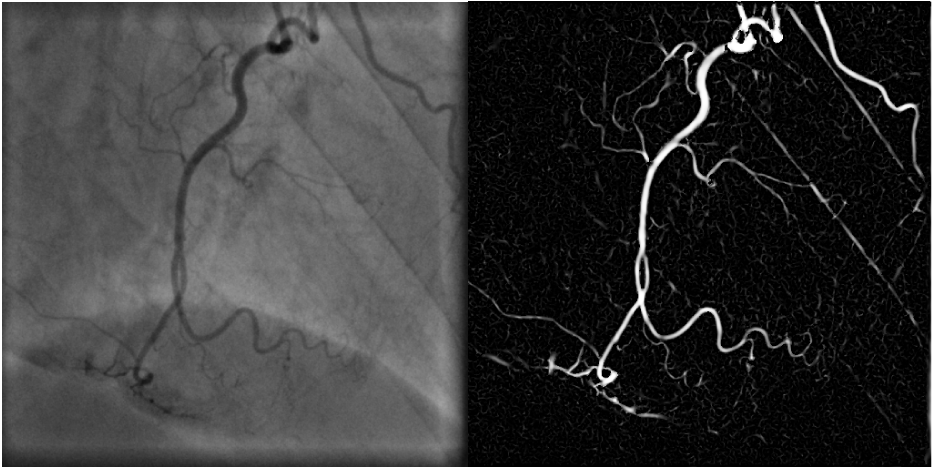
\includegraphics[width=3.0in]{possibilityimage.png}\\
  \caption{Possibility Image}\label{fig:possibilityimage}
\end{figure}

After having got the possibility image, we initialize another new
binary image for calculating centerlines. The pixels where the
extraction values are greater than zero are white while the others are
black. We compute the connectivity of the whole image using a cross
template so that line segments whose length are smaller than a typical
value are regarded as noise as well as many noisy points produced by
enhancement during MSR. After all these steps, we can reduce
over-extraction and noise as much as possible. The tracking result is
shown in Figure \ref{fig:lineseg_trace}.
\begin{figure}
  \centering
  % Requires \usepackage{graphicx}
  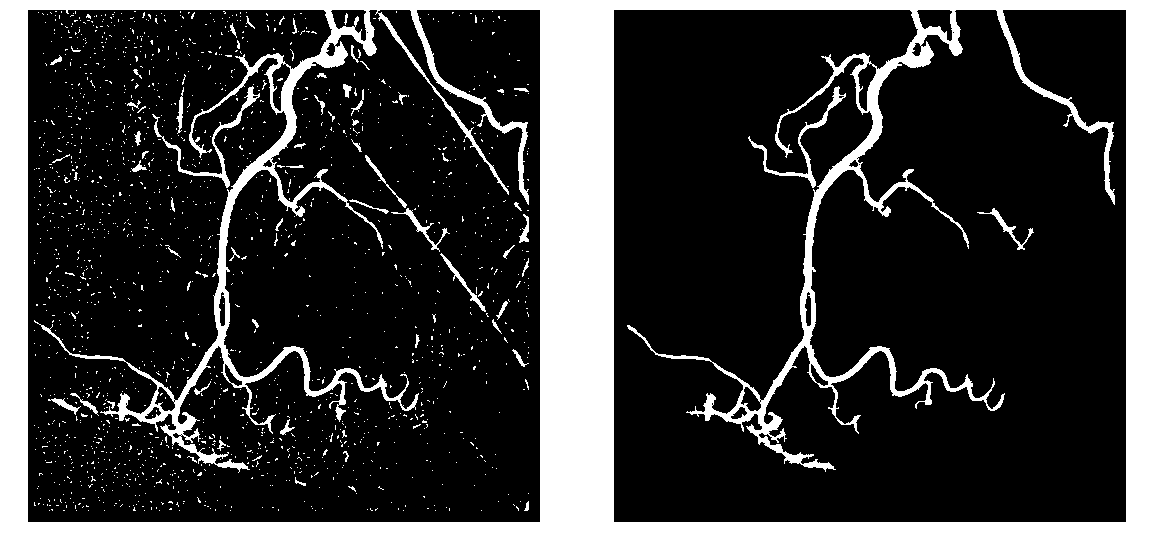
\includegraphics[width=3.0in]{lineseg_trace.png}\\
  \caption{Line Segment Trace Image}\label{fig:lineseg_trace}
\end{figure}

\subsubsection{Hysteresis-like Thresholding}
Hysteresis thresholding is to discard obvious non-vascular structures from
the result images while retaining the definite values. We use a histogram of
the image grey values to compute the quantiles of them as the basis of
thresholds. The low threshold is chosen low enough to obtain a slightly over
detection.
